\section{NNT Linear Combinations}


\frame{
    \frametitle{Reweighting using Full-Reco NNTs}
    \begin{columns}
        \begin{column}{0.4\textwidth}
            \begin{center} 
            {\tiny NNT Basis Set}

            \resizebox{0.2\textheight}{!}{ \begin{tabular}{ |l|l|l| }
                \hline
                \textbf {$\kappa_{2V}$} & \textbf {$\kappa_\lambda$} & \textbf {$\kappa_V$} \\
                \hline
                    1.  &   1. & 1.  \\
                    2.  &   1. & 1.  \\
                    1.5 &   1. & 1.  \\
   \rowcolor{green} 0.  &   1. & 0.5 \\
                    1.  &   0. & 1.  \\
                    1.  &  10. & 1.  \\
                \hline
            \end{tabular}}
            \end{center}

        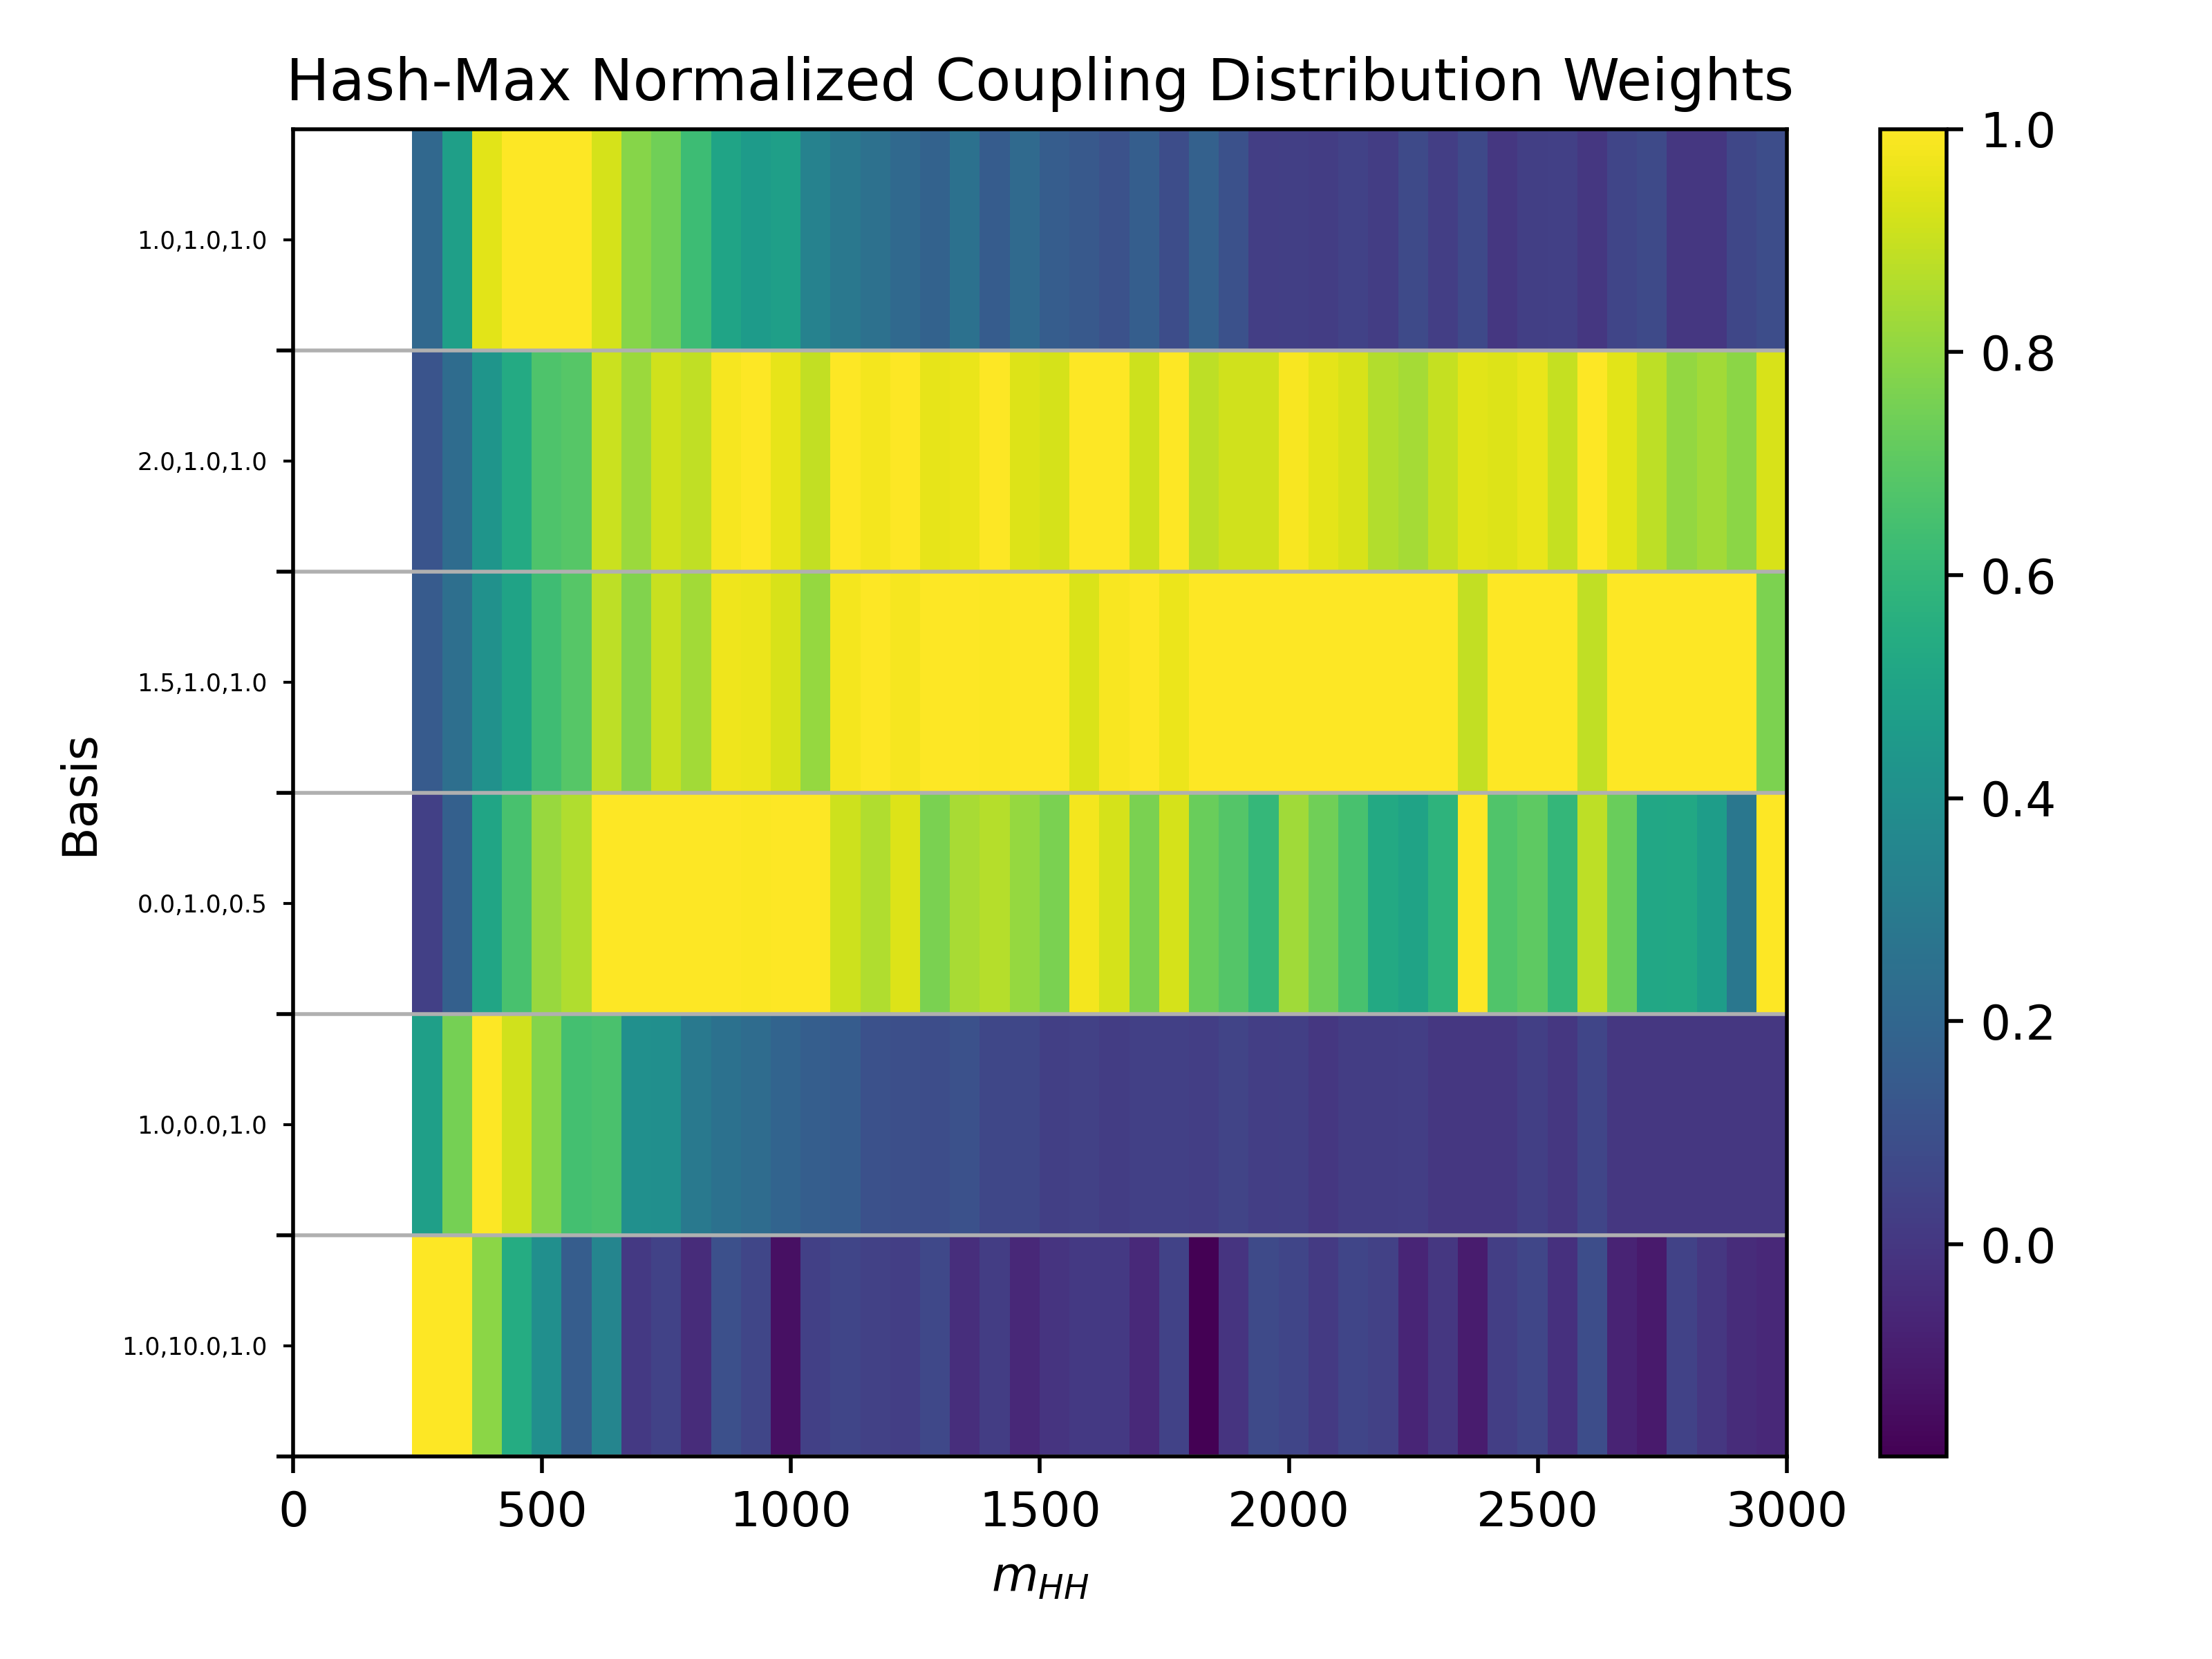
\includegraphics[width=\linewidth,height=\textheight,keepaspectratio]
            {coupling_scan_auto_chosen_reco_R0_hash_max}

        \end{column}
        \begin{column}{0.6\textwidth}
            Linear Combination Equation

            { \tiny Thanks for the extra sample Max! }
            \vspace{10mm}

            {\tiny $
A_{0} \left(2 \kappa_{2V}^{2} - \frac{124 \kappa_{2V} \kappa_{V}^{2}}{9} + \frac{61 \kappa_{2V} \kappa_{V} \kappa_{\lambda}}{9} + \frac{106 \kappa_{V}^{4}}{9} - \frac{17 \kappa_{V}^{3} \kappa_{\lambda}}{3} - \frac{\kappa_{V}^{2} \kappa_{\lambda}^{2}}{9}\right) + A_{1} \left(2 \kappa_{2V}^{2} - 8 \kappa_{2V} \kappa_{V}^{2} + 3 \kappa_{2V} \kappa_{V} \kappa_{\lambda} + 6 \kappa_{V}^{4} - 3 \kappa_{V}^{3} \kappa_{\lambda}\right) + A_{2} \left(- 4 \kappa_{2V}^{2} + 20 \kappa_{2V} \kappa_{V}^{2} - 8 \kappa_{2V} \kappa_{V} \kappa_{\lambda} - 16 \kappa_{V}^{4} + 8 \kappa_{V}^{3} \kappa_{\lambda}\right) + A_{3} \left(16 \kappa_{2V} \kappa_{V}^{2} - 16 \kappa_{2V} \kappa_{V} \kappa_{\lambda} - 16 \kappa_{V}^{4} + 16 \kappa_{V}^{3} \kappa_{\lambda}\right) + A_{4} \left(\frac{4 \kappa_{2V} \kappa_{V}^{2}}{5} - \frac{4 \kappa_{2V} \kappa_{V} \kappa_{\lambda}}{5} + \frac{\kappa_{V}^{4}}{5} - \frac{3 \kappa_{V}^{3} \kappa_{\lambda}}{10} + \frac{\kappa_{V}^{2} \kappa_{\lambda}^{2}}{10}\right) + A_{5} \left(- \frac{\kappa_{2V} \kappa_{V}^{2}}{45} + \frac{\kappa_{2V} \kappa_{V} \kappa_{\lambda}}{45} + \frac{\kappa_{V}^{4}}{45} - \frac{\kappa_{V}^{3} \kappa_{\lambda}}{30} + \frac{\kappa_{V}^{2} \kappa_{\lambda}^{2}}{90}\right)
$
}
        \end{column}
    \end{columns}
}

\displaythree{Validity of NNT Reweighting}
{ NNT reweighting results are not optimal, but will do for now

    \vspace{10mm}

    {\tiny Note that linear combination points do not have their errors shown here} 

}
{nnt_mHH_cvv0p0cl1p0cv1p0}
{nnt_mHH_cvv1p0cl2p0cv1p0}
{nnt_mHH_cvv4p0cl1p0cv1p0}
